\documentclass[reprint,showpacs,prb,nofootinbib,amsmath,amssymb]{revtex4-1}

\usepackage{listings}
\usepackage{graphicx}% Include figure files
\usepackage{dcolumn}% Align table columns on decimal point
\usepackage{bm}% bold math
\usepackage{breqn}
\usepackage{verbatim}   % useful for program listings
\usepackage{appendix}
\usepackage{hyperref}
\usepackage{footnote} 
\usepackage{url}

\begin{document}

\title{\textit{LineFit}: a Matlab Toolbox for 1D Line Fitting}
\author{Zhang Jiang}
%    X-ray Science Division\\
%    Advanced Photon Source\\
%    Argonne National Laboratory\\
%    zjiang@aps.anl.gov}
\date{\today}
%\date{October 21, 2016}
\maketitle
\tableofcontents
%\newpage

\section{Overview}

\verb|Linefit| is a toolbox for 1D line  fitting. In addition to over 30 built-in curve models, it allows combing those built-in model or customizing new models. As a class object, \verb|linefit|'s properties and methods allow one to customize fitting options, easily switch on/off parameters for fitting, evaluate models, and calculate model properties. It provides both script mode for batch processing and GUI mode for interactive fitting. 

\verb|Linefit| works on Matlab 2015b or later. It requires Matlab Optimization Toolbox for \verb|lsqcurvefit| solver. 

\section{Installation}

Add the \verb|linefit| directory to Matlab search path either from the \verb|Set Path| in Matlab Home tab or run \verb|>>addpath <your path>/linefit| in the command window. If Voigt distribution function is used, one needs add the Faddeeva~\cite{Faddeeva} sub-directory. 
	
\section{Usage}

We use `curve' to denote the model for fitting and 'bkgd' to denote the model for background. They are stored as fields in private property \verb|linefit.ModelBase|
\begin{align}
	\mbox{CurveModel} 	&: \mbox{[1x1 struct]} \nonumber \\
	\mbox{BkgdModel}	&: \mbox{[1x1 struct]} \nonumber 
\end{align}
Each field itself is a structure consisting of model function handle, number of parameters, start values, lower and upper bounds, fit flags, and etc. For example, \verb|CurveModel| has default fields:
\begin{align}
	\mbox{ModelFcnHandle} 	&: \mbox{@linefit.lorentzian} \nonumber \\
	\mbox{NOfParams}	&: \mbox{[3 1]} \nonumber \\
	\mbox{StartParams}	&: \mbox{[3x1 double]} \nonumber \\
	\mbox{LowerBounds}	&: \mbox{[3x1 double]} \nonumber \\
	\mbox{UpperBounds}	&: \mbox{[3x1 double]} \nonumber \\
	\mbox{FitFlags}		&: \mbox{[3x1 double]} \nonumber \\
	\mbox{ModelName}	&: \mbox{`Cauchy/Lorentzian'} \nonumber \\	
	\mbox{ModelUsage}	&: \mbox{`lorentzian(x,[amp,x0,gamma])'} \nonumber \\
	\mbox{FitStdErrors}	&: \mbox{[3x1 double]} \nonumber 					
\end{align}
\verb|FitFlags| is a logical matrix with 1 for fitting and 0 fixed parameters. \verb|FitStdErrors| is a place holder to store the standard deviations after fitting; and its initial value is set to -1 (also an indicator for non-fitting parameters). \verb|ModelBase| is a private property that cannot be directly changed by users. Instead, the curve and background models can be indirectly changed to other built-in models by setting properties \verb|CurveModelIndex| and \verb|BkgdModelIndex| (see Appendix~\ref{app:properties} for details). After a new \verb|linefit| object is created and loaded with 2-column data into property \verb|Data|, \verb|ModelBase| is automatically copied to a public property \verb|Model|, whose field values such as start values, lower and upper bounds, and fit flags can be directly changed. Such way of managing models allows an easy setup for models with multiple curves of the same curve type (e.g. crystallography profiles with multiple peaks). This is achieved simply by adding or reducing number of curves in the \verb|Model.CurveMode| (via method \verb|addcurves| and \verb|reducecurves|) while keeping the base curve model unchanged in \verb|ModelBase|.

There is no better way to demonstrate than going through examples. 

\subsection{Script Mode}

\subsubsection{Fitting a double-peak profile}
Create a \verb|linefit| object and load data
\begin{eqnarray*}
&&\verb|foo=load(`demo_doublpeak.dat')| \\
&&\verb|a=linefit(foo)|
\end{eqnarray*}

Instead of default settings of Lorentzian curve mode and no background, we two Gaussian curves and constant background
\begin{eqnarray*}
	&&\verb|a.CuveModelIndex=4 % Gaussian| \\
	&&\verb|a.BkgdModelIndex=1 % constant background| \\
	&&\verb|a=addcurves(a,1)   % add a curve to the end|
\end{eqnarray*}
After method \verb|addcurves| appends another Gaussian curve to the model, a new \verb|linefit| is returned and assigned back to the original object \verb|a|. 

To preview the model with start parameter values
\begin{eqnarray*}
&&\verb|plot(a)| \text{  or } \verb|plot(a,`preview')|
\end{eqnarray*}

\verb|Linefit| uses built-in Matlab solver \verb|lsqcurvefit|. The optimization options are identical to those for \verb|lsqcurvefit|, and can be accessed or changed in property \verb|FitOptions|.

To start fitting,
\begin{eqnarray*}
	&&\verb|a=startfit(a)|
\end{eqnarray*}
Fit results, such as fitted parameters and their standard deviations, squared norm of the residual, residuals, exit flag (reason to stop fitting), output (information about fitting process), Jacobian at the solution, and etc., are temporarily saved in \verb|FitOutput| waiting for acceptance or rejection.
\begin{eqnarray*}
	&&\verb|plot(a,`fit')|
\end{eqnarray*}
plots the the fitted curve on the raw data, as well as the residuals. 
\begin{eqnarray*}
	&&\verb|a=acceptfit(a)|
\end{eqnarray*}
accepts fit result and updates start values (\verb|StartParams|) and standard deviations (\verb|FitStdErrors|) for both \verb|CurveModel| and \verb|BkgdModel|. Nothing needs to be done to reject.

You can then get the model properties (if defined for the model) such as mean, variance, median, skewness, kurtosis, and etc, either analytically or numerically,
\begin{eqnarray*}
	&&\verb|getmodelprops(a) 	% analytical method| \\
	&&\verb|getmodelprops(a,linspace(-100,100,1000))| \\
	&&\verb|                  % numerical method|
\end{eqnarray*}

You may evaluate the model (calculate the y values) on provided x data or any list of x data by
\begin{eqnarray*}
	&&\verb|y=evalmodel(a) 	% on provided x data| \\
	&&\verb|y=evalmodel(a,-100:0.1:100)|\\
	&&\verb|	               % on other x data|
\end{eqnarray*}
Note that because \verb|getmodelprops| and \verb|evalmodel| use the start values (see Appendix~\ref{app:methods}), you need to accept fit result first if you wish to get the properties and model evaluations on fit result.

\subsubsection{Customized or combined curve models}\label{sec:custommodel}

Now we demonstrate how to create a customized or combined curve model. 

Still use the data from the last example. Suppose the customized curve model is
\begin{equation}
f(x)=A\exp\left(-|x-x_0|^3/b\right) \nonumber
\end{equation}
We need to first create the custom model (see Appendixe~\ref{app:methods} for usage details) by
\begin{widetext}
\begin{eqnarray*}
\verb|a.CustomCurveModel=linefit.createmodel(|&&\verb|@(x,p)p(1)*exp(-abs(x-p(2)).^3/p(3)),| \\
&&\verb|3,[1,0,5],[0,-1,0],[100,10,Inf],[1,1,1])|
\end{eqnarray*}
\end{widetext}
where the 1st argument is an anonymous function handle whose expression must be vectorized (e.g. using the `.' for the power, multiplication, division etc), the 2nd argument is the total number of parameters, and the 3rd-6th arguments are start values, lower bounds, upper bounds, and fit flags. The 3rd-6th arguments can be empty [ ] to use the default settings: random values for start values, -Inf's for lower bounds, Inf's for upper bounds, and 1s for fit flags. One can also create a customized model by working out the function in a Matlab .m file. Let's say file \verb|myfun.m| has the function defined by the following lines 
\begin{eqnarray*}
	&&\verb|function y=myfun(x,p)| \\
	&&\verb|y=p(1)*exp(-abs(x-p(2)).^3/p(3));|
\end{eqnarray*}
This file has to be in the current working directory or wherever Matlab can see it from its path settings. We then create the model by
\begin{widetext}
	\begin{eqnarray*}
		\verb|a.CustomCurveModel=linefit.creatmodel(|&&\verb|@(x,p)myfun,3,[1,0,5],[0,-1,0],[100,10,Inf],[1,1,1])|
	\end{eqnarray*}
\end{widetext}
The customized model is then loaded to \verb|ModelBase| by setting \verb|CurveModeIndex| to -2.
\begin{eqnarray*}
	&&\verb|a.CurveModelIndex=-2;|
\end{eqnarray*}
We then add one more curve of the same model and start the fitting
\begin{eqnarray*}
&&\verb|a=addcurves(a,1);| \\
&&\verb|a=a.startfit;|
\end{eqnarray*}
Note that analytical model properties are not defined for customized models; instead, use numerical method.

If one Lorentzian and one Gaussian are desired to model the double peak data, we can combine these two built-in models by creating a multi-model
\begin{eqnarray*}
	\verb|a.CustomCurveModel=|&&\verb|a.creatmodel([1,4],[],|\\
	&&\verb|[],[],[],[],[])|
\end{eqnarray*}
where the 1st argument \verb|[1,4]| are the index for Lorentzian and Gaussian. The number of parameters is automatically set to the total number of parameters of these two built-in models; thus the 2nd argument is left empty. The other arguments are also left empty to use the default settings. We then load this multi-model to \verb|ModelBase| by setting the model index to -1
\begin{eqnarray*}
	&&\verb|a.CurveModelIndex=-1;| 
\end{eqnarray*}
If you get to this step by continuing the last example where two curves are used, you need to reduce the number of curves to one, because the multi-model itself is a double-peak profile although it is considered as a one curve model.
\begin{eqnarray*}
\verb|a=reducecurves(a,2)|
\end{eqnarray*}
where the 2nd argument is the index(es) of the current curves to be removed in \verb|Model.CurveModel|.

Customized background model can be created in the same way as the customized curve model, but one cannot combine built-in background models. Multiple background models of the same type are not allowed either.

\subsection{GUI Mode}
\begin{figure*}
	\centering
	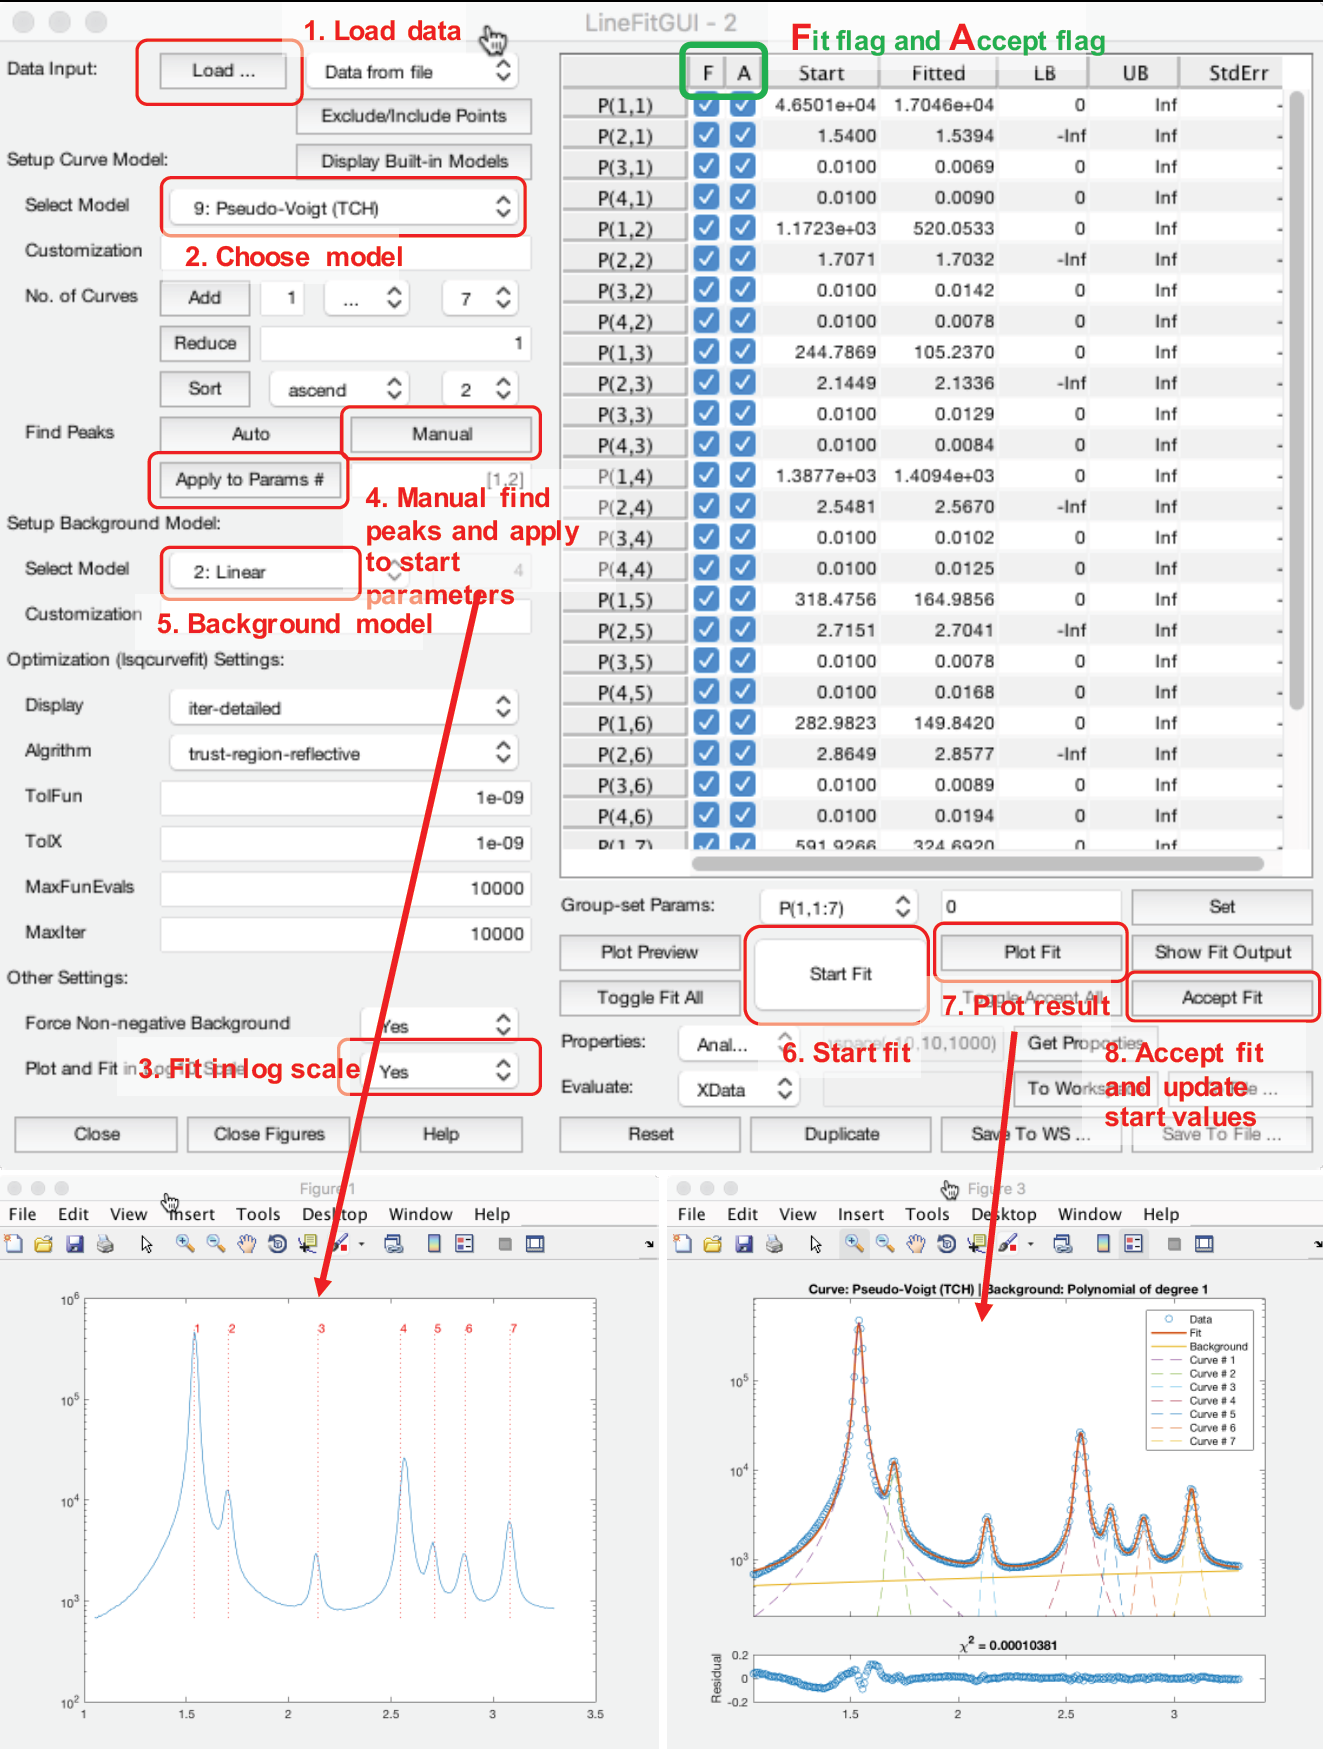
\includegraphics[width=.8\linewidth]{fig}
	\caption{Top: GUI; Bottom left: manually find peaks; Bottom right: plot after fitting.}
	\label{fig:fig}
\end{figure*}	

Although \verb|linefit| toolbox is fully functional in the script model, a GUI interface (\verb|linefitgui|) provides a faster access if there are not too many data sets to be managed. Let's demonstrate with an example. Start GUI and load data
\begin{eqnarray*}
	&&\verb|foo=load(`demo_xtal.data');| \\ 
	&&\verb|linefitgui(foo)|
\end{eqnarray*}
One also start GUI first by \verb|linefitgui| and load data from there. Complete the fitting by following the steps in Fig.~\ref{fig:fig}.

To use customized model or multi-mode In GUI mode, enter the arguments only separated by commas in the Customization edit boxes, e.g.,
\begin{eqnarray*}
	&&\verb|@(x,p)p(1)*exp(-abs(x-p(2)).^3/p(3)),| \\
	&&\verb|3,[1,0,5],[0,-1,0],[100,10,Inf],[1,1,1]|
\end{eqnarray*}
or
\begin{eqnarray*}
\verb|[1,4],[],[],[],[],[],[]|
\end{eqnarray*}
There is no need to enter the method name \verb|createmodel|. Then use the Select Model popupmenu to change the model index to customized model or multi-model.

\appendix
\appendixpage
\addappheadtotoc
\section{List of \textbf{linefit} properties}\label{app:properties}
In Matlab command window, type \verb"linefit" to view the default properties of a \verb"linefit" object.
\allowdisplaybreaks{
\begin{align}
\mbox{Data} 				&: \mbox{[]} \nonumber \\
\mbox{CurveModelIndex}		&: \mbox{1} \nonumber \\
\mbox{BkgdModelIndex}       &: \mbox{0} \nonumber \\
\mbox{CustomCurveModel}     &: \mbox{[1x1 struct]}  \nonumber \\
\mbox{CustomBkgdModel}      &: \mbox{[1x1 struct]}  \nonumber \\
\mbox{Model}         		&: \mbox{[1x1 struct]}  \nonumber \\
\mbox{FlagNonNegBkgd}       &: \mbox{1}  \nonumber \\
\mbox{FlagLogScale}         &: \mbox{0}  \nonumber \\
\mbox{FitOptions}     		&: \mbox{[1x1 optim.options.Lsqcurvefit]} \nonumber \\
\mbox{FitOutput}            &: \mbox{[1x1 struct]}  \nonumber \\
\mbox{ModelList}            &: \mbox{[1x30 struct]}  \nonumber \\
\mbox{PeaksFound}           &: \mbox{[]}  \nonumber \\
\mbox{ModelBase}            &: \mbox{[1x1 struct]}  \nonumber \\
\mbox{NOfModelCurves}       &: \mbox{1}  \nonumber
\end{align}
}

Public properties that are independent and can be set or accessed by users are
\begin{itemize}
\item \verb"Data": (Public) Input data. Must be a 2-column double or single type data [XData,YData].
\item \verb"CurveModelIndex": (Public) Index of curve models. In Matlab command window, type \verb"linefit.getmodellist" to display all models, usage and initial parameters.
\item \verb"BkgdModelIndex": (Public) Index of background models. -2/-1/[0]/1/2/3/../N: Custom/Power/[No]/Constant/Linear/Quadratic/.../Polynomial of degree N.
\item \verb"CustomCurveModel": (Public) Structure to store custom or multi curve model. Can be created with \verb"createmodel" method.
\item \verb"CustomBkgdModel": (Public) Structure to store custom background model. Can be created with \verb"createmodel" method.
\item \verb"Model": (Public) Complete fit model including both curve and background models (\verb"CurveModel" and \verb"BkgdModel").
\item \verb"FlagNonNegBkgd": (Public) Flag to force a non-negative background. 0/[1]: no/[yes]. 
\item \verb"FlagLogScale": (Public) Flag to fit in log scale for YData. [0]/1: [no]/yes.
\item \verb"FitOptions": (Public) Optimization options for solver \verb"lsqcurvefit". See Matlab help or documentation for \verb"lsqcurvefit".
\item \verb"FitOutput": (Public) Structure to store fitting result.
\item \verb"ModelList": (Private) Definition of built-in models.
\item \verb"PeaksFound": (Private) Peak value and positions ([Y, X]) for the initialization of peak-shaped models.
\item \verb"ModelBase": (Private) Base curve model and background model for fitting. \verb|ModelBase.CurveModel| is replicated to \verb"Model.CurveModel" if multiple identical curves are used (\verb|NOfModelCurves|). \verb|ModelBase| can be changed only via \verb|CurveModelIndex|.
\item \verb"NOfModelCurves": Number of curves. It can be increased or decreased by methods \verb|addcurves| and \verb|reducecurves|.
\end{itemize}

\section{List of \textbf{linefit} methods}\label{app:methods}

Dynamic methods can be called in two ways: \verb|obj.MethodName(argument1,...)| or \verb|MethodName(obj,argument1,...)|. The 2nd way will be adopted below. Static methods can be called like the 1st way for dynamic methods; they can also be directly called by \verb|linefit.MethodName(argument1,...)| without first creating an object.

\begin{itemize}
\item \verb|linefit| (dynamic): Create a new \verb"linefit" object.

\verb|obj=linefit| creates an empty object. 

\verb|obj=linefit(data)| creates an object with \verb|data| and default settings.

\item \verb|addcurves| (dynamic): Add curves of identical \verb|ModelBase.CurveModel| to \verb|Model.CurveModel|.

\verb|obj2=addcurves(obj1)| adds one curve to the end. 

\verb|obj2=addcurves(obj1,n)| adds \verb|n| curves to the end. 

\verb|obj2=addcurves(obj1,n,pos)| adds \verb|n| curves to position \verb|pos|. \verb|pos| must be a non-zero integer. The value of \verb|pos| (i.e. \verb"|pos|") is the position; the sign of \verb|pos| is the direction (i.e. + means an insertion after \verb"|pos|" and - means an insertion before \verb"|pos|"). 

This method creates a new object \verb|obj2|. Setting \verb|obj2| to \verb|obj1| as the output argument avoids creating a new object.

\item \verb|reducecurves| (dynamic): Reduce curves from \verb|Model.CurveModel|.

\verb|obj2=reducecurves(obj1)| reduces the last one curve in the list end. 

\verb|obj2=reducecurves(obj1,index)| reduces curves of position \verb|index|. \verb|index| must be a scalar or a vector, e.g., [2,5:7] removes curve \#2, \#5, \#6, and \#7.

\item \verb|sortcurves| (dynamic): Sort the order of curves in \verb|Model.CurveModel|.

\verb|obj2=sortcurves(obj1,row)| sorts the curves with default \verb|mode=`ascend'| according to the values in row number \verb|row|, i.e. the index position of the parameters. For example, \verb|row=2| sorts the order of the two curves by the values of the parameters values in \verb|p(2)| in the example in Section~\ref{sec:custommodel}.

\verb|obj2=sortcurves(obj1,row,mode)| sorts with \verb|mode=`ascend'| or \verb|`descent'|.

\item \verb|startfit| (dynamic): Start fitting.

\verb|obj2=startfit(obj1)| starts fitting and stores fit result in \verb|obj2.FitOutput|.

\item \verb|acceptfit| (dynamic): Accept and pass fit result to fields \verb|StartParams| and \verb|FitStdErrors| in \verb|Model.CurveModel| and \verb|Model.BkgdModel|.

\verb|obj2=accetpfit(obj1)| returns to a new object \verb|obj2|.

\item \verb|evalmodel| (dynamic): Evaluate \verb|Model|.

\verb|y=evalmodel(obj)| evaluates using XDATA in \verb|obj.Data| and returns values to \verb|y|.

\verb|y=evalmodel(obj,XV)| evaluates on a vector \verb|XV|.

\verb|[y,iy]=evalmodel(obj,...)| also returns the values for each curve to \verb|iy|.

\verb|[y,iy,bkgd]=evalmodel(obj,...)| also returns the background values to \verb|bkgd|.

\item \verb|plot| (dynamic): Plot model calculations with start parameters or fitted parameters.

\verb|plot(obj)| preview model calculations using parameters in \verb|obj.Model|.

\verb|plot(obj,mode)| plots model calculations when \verb|mode=`preview'|, and fitting result when \verb|mode=`fit'|. Default is \verb|mode=`preview'|. The \verb|`fit'| mode also plots the residual and labels the Pearson's $\chi2$, which are defined by 
\begin{eqnarray*}
\mathrm{Residual}(x_i)&=&f(x_i)-y_i \\
\chi^2&=&\sum_{i}^{n}\frac{\left[f(x_i)-y_i\right]^2}{y_i}
\end{eqnarray*}

\verb|hlines=plot(obj,...)| returns the handle of the plotted data line.

\item \verb|findpeakauto| (dynamic): Automatically search for peaks in \verb|Data|.

\verb|obj2=findpeakauto(obj1)| uses function \verb|peakfinder.m| to find peaks~\cite{peakfinder} and stores them to \verb|obj2.peaksfound|.

\verb|obj2=findpeakauto(obj1,arg1,arg2...)| uses arguments defined in \verb|peakfinder|.

\item \verb|findpeakmanual| (dynamic): Manually and interactively search for peaks.

\verb|obj2=findpeakmanual(obj1)| uses interactive tool \verb|getpts| (requires Matlab Image Processing Toolbox) to identify peaks.

\item \verb|getmodelprops| (dynamic): Get curve model properties such as mean, variance, FWHM, skewness, kurtosis, and etc.

\verb|s=getmodelprops(obj)| gets curve model properties using analytical method and returns to a structure \verb|s|. 

\verb|s=getmodelprops(obj,XV)| numerically calculates model properties using x values \verb|XV|. \verb|XV| must be a vector. Suppose function $f(x)$ is normalized, i.e., $\int{f(x)dx}=1$. Mean value is then calculated by with Matlab numerical integration function \verb|trapz|,
\begin{equation}
\mu=\int{xf(x)dx}; \nonumber
\end{equation}
the variance (the 2nd central momentum) is calculated by
\begin{equation}
\mu_2=\int{(x-\mu)^2f(x)dx}; \nonumber
\end{equation}
skewness is calculated by
\begin{equation}
\gamma_1=\frac{\mu_3}{\sigma^3},\nonumber
\end{equation}
where $\mu_3=\int{(x-\mu)^3f(x)dx}$ is the 3rd central momentum, and $\sigma=\sqrt{\mu_2}$ is the standard deviation; and excess kurtosis is calculated by
\begin{equation}
\gamma_2=\frac{\mu_4}{\sigma^4}-3,\nonumber
\end{equation}
where $\mu_4=\int{(x-\mu)^4f(x)dx}$ is the 4th central momentum.

\item \verb|applypeaks| (dynamic): Pass peak values and positions in \verb|PeaksFound| to \verb|Model.CurveModel.StartParams|, and set the number of curves to the number of peaks found.

\verb|obj2=applypeaks(obj1)| passes to the 1st and 2nd input parameters (peak amplitudes and positions) for built-in curve models \#1-18 (peak-shaped models).

\verb|obj2=applypeaks(obj1,rows)| passes to \verb|rows| of \verb|Model.CurveModel.StartParams|. \verb|rows| must be a two-element vector with the 1st value for peak amplitude row and 2nd  value for peak location row. For example, \verb|rows|=[3,4] means that, in the model, the 3rd parameter is the peak amplitude and the 4th  parameter is the peak location (x value).

\item \verb|createmodel| (static): Create model structure for \verb|linefit| object

\verb|s=linefit.createmodel(fcn_handle,nofp,| \verb|startparams,lowerbounds,upperbounds,fitflags)|. \verb|fcn_handle| is the function handle for the model. \verb|nofp| is the number of total parameters in the model. \verb|startparams|, \verb|lowerbounds|, and \verb|upperbounds| are initial parameters, lower and upper bounds for the fitting. \verb|fitflags| is logical flags (false/true or 0/1) to indicate whether the parameter is to be fixed or fitted. \verb|startparams|, \verb|lowerbounds|, \verb|upperbounds|, and \verb|fitflags| must be either vector of dimension \verb|nofp|$\times1$, or empty \verb|[]| for default values (random values for \verb|startparams|,
-Inf, Inf and 1 for \verb|lowerbounds|, \verb|upperbounds|, and \verb|fitflags|).

\verb|fcn_handle| must have the format \verb|@(x,p)UserFcn(x,p)| where \verb|x| is the input x value, \verb|p| is a vector of parameters; or it can be an anonymous function, e.g.,
\verb|f=@(x,p)p(1)+p(2)*x+p(3)*sin(x)| (which gives a value  of 3.7296 when
x=4 and p=[2,1,3], i.e. \verb|f(4,[2,1,3])=3.7296|).

For a multi-model (\verb|CurveModelIndex=-1|) where the \verb|Model.CurveModel| is constructed as a sum of built-in models, use \verb|s=createmodel(models,[],startparams,| \verb|lowerbounds,upperbounds,fitflags)|, where \verb|models| is a list of indexes of built-in models, e.g., \verb|models[1,4,13]| constructs a multi-model using the sum of Lorentzian (model \#1), Gaussian (model \#4) and Voigt (model \#13). The default of \verb|nofp| is automatically set to the total number of parameters of these built-in models.

\verb|s=createmodel(...,fitflags,modelname)| takes a name (string) for the model. It is automatically set to empty if not specified, or forced to be built-in model indexes when \verb|CurveModelIndex=-1|.

\verb|s=createmodel(...,modelname, modelusage)| takes usage instructions (string) for the model.

\item \verb|lineprops| (static): Numerically calculate line properties.

\verb|s=obj.lineprops(data)| or \verb|s=linefit.| \verb|lineprops(data)| calculates properties for a 2-column \verb|data|. It outputs a structure \verb|s| with fields: \verb|s.area| for numerically integrated area (using Matlab \verb|trapz| function); \verb|s.peak| for the peak X, Y values, and position index; \verb|s.mean|, \verb|s.variance|, \verb|s.skewness|, \verb|s.kurtosis|, and \verb|s.fwhm| for mean, variance, skewness, kurtosis, and full-width-of-half-maximum (FWHM); and \verb|s.fwhm_x| for the center position of FWHM.

\item \verb|getmodellist| (static): Get the list of built-in models with name, usage, inital parameters, bounds and etc.

\verb|s=obj.getmodellist| or \verb|s=linefit.| \verb|getmodellist| returns to a table \verb|s|.

\end{itemize}

\section{List of \textbf{linefit} built-in curve models}\label{app:builtin}

These functions are defined as static methods, which can be called the same way as other \verb|linefit| static methods. General usage of these functions is \verb|y=linefit.function_name(x,p)| or \verb|[y,props]=| \verb|linefit.function_name(x,p)|, where \verb|p| is the parameter vector defined below, and \verb|props| is a structure for model properties, such as mean, variance and etc.

Note that not all functions have analytical formulas for mean, variance, skewness, kurtosis, or FWHM. Although one may force a calculation of these properties by numerically evaluating the model (see \verb|linefit| method \verb|getmodelprops|), properties such as skewness and kurtosis may not be mathematically defined at all.

Most distribution functions are normalized unless explicitly claimed.

There are 31 built-in models. Models \#1-18 are distribution functions with support $(-\infty,\infty)$; models \#19-28 are distribution functions with half-infinity support; the rest of the models are other profile functions.

\begin{enumerate}
\item \verb|lorentzian(x,[A,x0,gamma])| Lorentzian or Cauchy distribution function

\verb|A|: amplitude, \verb|x0|: location, \verb|gamma| ($\gamma>0$): scale or HWHM (half-width-of-half-maximum).
\begin{equation}
f(x)=A\frac{1}{\pi\gamma}\left[1+\left(\frac{x-x_0}{\gamma}\right)^2\right]^{-1} \nonumber
\end{equation}
\begin{align}
	\mbox{mode}      	&: \mbox{$x_0$}  \nonumber \\
	\mbox{median}       &: \mbox{$x_0$}  \nonumber \\
	\mbox{fwhm} 		&: \mbox{$2\gamma$}  \nonumber
\end{align}

\item \verb|ilorentzian(x,[A,x0,gamma])| Intermediate Lorentzian distribution function~\cite{ilorentzian}

\verb|A|: amplitude, \verb|x0|: location, \verb|gamma| ($\gamma>0$): scale.
\begin{equation}
f(x)=A\frac{\sqrt{2^{\frac{2}{3}}-1}}{2\gamma}\left[1+(2^{\frac{2}{3}}-1)\left(\frac{x-x_0}{\gamma}\right)^2\right]^{-\frac{3}{2}} \nonumber
\end{equation}
\begin{align}
	\mbox{mode}      	&: \mbox{$x_0$}  \nonumber \\
	\mbox{median}       &: \mbox{$x_0$}  \nonumber \\	
	\mbox{fwhm} 		&: \mbox{$2\gamma$}  \nonumber
\end{align}

\item \verb|mlorentzian(x,[A,x0,gamma])| Modified Lorentzian distribution function~\cite{mlorentzian}

\verb|A|: amplitude, \verb|x0|: location, \verb|gamma| ($\gamma>0$): scale.
\begin{equation}
f(x)=A\frac{2\sqrt{\sqrt{2}-1}}{\pi\gamma}\left[1+(\sqrt{2}-1)\left(\frac{x-x_0}{\gamma}\right)^2\right]^{-2} \nonumber
\end{equation}
\begin{align}
	\mbox{mode}      	&: \mbox{$x_0$}  \nonumber \\
	\mbox{median}       &: \mbox{$x_0$}  \nonumber \\
	\mbox{fwhm} 		&: \mbox{$2\gamma$}  \nonumber
\end{align}

\item \verb|gaussian(x,[A,x0,sigma])| Gaussian or normal distribution function

\verb|A|: amplitude, \verb|x0|: location, \verb|sigma| ($\sigma>0$): scale or standard deviation.
\begin{equation}
f(x) = A\frac{1}{\sigma\sqrt{2\pi}}\exp\left[-\frac{(x-x_0)^2}{2\sigma^2}\right] \nonumber
\end{equation}
\begin{align}
	\mbox{mean} 		&: \mbox{$x_0$} \nonumber \\
	\mbox{variance}		&: \mbox{$\sigma^2$} \nonumber \\
	\mbox{skewness}     &: \mbox{$0$} \nonumber \\
	\mbox{kurtosis}     &: \mbox{$0$}  \nonumber \\
	\mbox{mode}      	&: \mbox{$x_0$}  \nonumber \\
	\mbox{median}       &: \mbox{$x_0$}  \nonumber \\
	\mbox{fwhm} 		&: \mbox{$2\sqrt{2\log(2)}\sigma$}  \nonumber
\end{align}

\item \verb|generalizednorm1(x,[A,a,b,c])| Generalized normal distribution function version 1~\cite{generalizednorm1}

\verb|A|: amplitude, \verb|a|: location, \verb|b|$>0$: scale, \verb|c|$>0$: shape. 
\begin{equation}
f(x)=A\frac{c}{2b\Gamma(1/c)}\exp\left[-\left(\frac{\left|x-a\right|}{b}\right)^c\right] \nonumber
\end{equation}
\begin{align}
	\mbox{mean} 		&: \mbox{$a$} \nonumber \\
	\mbox{variance}		&: \mbox{$\frac{b^2\Gamma(3/c)}{\Gamma(1/c)}$} \nonumber \\
	\mbox{skewness}     &: \mbox{$0$} \nonumber \\
	\mbox{kurtosis}     &: \mbox{$\frac{\Gamma(5/c)\Gamma(1/c)}{\Gamma(3/c)^2}-3$}  \nonumber \\
	\mbox{mode}      	&: \mbox{$a$}  \nonumber \\
	\mbox{median}       &: \mbox{$a$}  \nonumber
\end{align}

\item \verb|laplace(x,[A,a,b])| Laplace distribution function~\cite{McLaughlin}

\verb|A|: amplitude, \verb|a|: location, \verb|b|$>0$: scale. 
\begin{equation}
f(x)=A\frac{1}{2b}\exp\left(-\frac{\left|x-a\right|}{b}\right) \nonumber
\end{equation}
\begin{align}
	\mbox{mean} 		&: \mbox{$a$} \nonumber \\
	\mbox{variance}		&: \mbox{$2b^2$} \nonumber \\
	\mbox{skewness}     &: \mbox{$0$} \nonumber \\
	\mbox{kurtosis}     &: \mbox{$3$}  \nonumber \\
	\mbox{mode}      	&: \mbox{$a$}  \nonumber \\
	\mbox{median}       &: \mbox{$a$}  \nonumber
\end{align}

\item \verb|logistic(x,[A,a,b])| Logistic distribution function~\cite{McLaughlin}

\verb|A|: amplitude, \verb|a|: location, \verb|b|$>0$: scale. 
\begin{equation}
f(x)=A\frac{1}{b}\exp\left(-\frac{x-a}{b}\right)\left[1+\exp\left(-\frac{x-a}{b}\right)\right]^{-2} \nonumber
\end{equation}
\begin{align}
	\mbox{mean} 		&: \mbox{$a$} \nonumber \\
	\mbox{variance}		&: \mbox{$\pi^2b^2/3$} \nonumber \\
	\mbox{skewness}     &: \mbox{$0$} \nonumber \\
	\mbox{kurtosis}     &: \mbox{$7/5$}  \nonumber \\
	\mbox{mode}      	&: \mbox{$a$}  \nonumber \\
	\mbox{median}       &: \mbox{$a$}  \nonumber
\end{align}

\item \verb|pearsonVII(x,[A,a,b,c])| Pearson type VII or student' t distribution function~\cite{McLaughlin,pearsonVII}

\verb|A|: amplitude, \verb|a|: location, \verb|b|$>0$: scale, \verb|c|$>0$: shape (degree of freedom).
\begin{equation}
f(x)=A\frac{\Gamma(\frac{c+1}{2})}{b\sqrt{\pi c}\Gamma(\frac{c}{2})}\left[1+\frac{1}{c}\left(\frac{x-a}{b}\right)^2\right]^{-\frac{c+1}{2}} \nonumber
\end{equation}
\begin{align}
	\mbox{mean} 		&: \mbox{$a$ for $c>1$, otherwise undefined} \nonumber \\
	\mbox{variance}		&: \mbox{$\frac{b^2c}{c-2}$ for $c>2$, $\infty$ for $1<c\leq2$,} \nonumber \\
	\mbox{} 			&  \mbox{otherwise undefined} \nonumber \\
	\mbox{skewness}     &: \mbox{$0$ for $c>3$, otherwise undefined} \nonumber \\
	\mbox{kurtosis}     &: \mbox{$\frac{6}{c-4}$ for $c>4$, $\infty$ for $2<c\leq4$,} \nonumber \\
	\mbox{} 			&  \mbox{otherwise undefined} \nonumber \\	
	\mbox{mode}      	&: \mbox{$a$}  \nonumber \\
	\mbox{median}       &: \mbox{$a$}  \nonumber
\end{align}

\item \verb|pseudovoigtTCH(x,[A,x0,sigma,gamma])| Pseudo-Voigt type TCH distribution function~\cite{pseudovoigtTCH}

\verb|A|: amplitude, \verb|x0|: location, \verb|sigma| ($\sigma>0$): scale (standard deviation) of the Gaussian for convolution, \verb|gamma| ($\gamma>0$): scale (HWHM) of the Lorentzian for convolution.
\begin{equation}
f(x;\Gamma)=A\left[(1-\eta_L)f_G(x;\gamma_G)+\eta_L f_L(x;\sigma_L)\right], \nonumber
\end{equation}
where $\Gamma$ is the approximated FWHM of Voigt given by
\begin{eqnarray}
\Gamma&=&(\Gamma_{GV}^5+2.69269\Gamma_{GV}^4\Gamma_{LV}+2.42843\Gamma_{GV}^3\Gamma_{LV}^2 \nonumber \\
&+&4.47163\Gamma_{GV}^2\Gamma_{LV}^3+0.07842\Gamma_{GV}\Gamma_{LV}^4+\Gamma_{LV}^5)^{\frac{1}{5}}. \nonumber
\end{eqnarray}
with $\Gamma_{GV}=2\sqrt{2\log(2)}\sigma$ and $\Gamma_{LV}=2\gamma$; $f_L(x)$ is a Lorentzian given by
\begin{equation}
f_L(x;\gamma_L)=\frac{1}{\pi\gamma_L}\left[1+\left(\frac{x-x_0}{\gamma_L}\right)^2\right]^{-1}, \nonumber
\end{equation}
with $\gamma_L=\Gamma/2$; $f_G(x)$ is a Gaussian given by
\begin{equation}
f_G(x) = \frac{1}{\sqrt{2\pi\sigma_G^2}}\exp\left[-\frac{(x-x_0)^2}{2\sigma_G^2}\right], \nonumber
\end{equation}
with $\sigma_G=\Gamma/(2\sqrt{2\log(2)})$; 
$\eta_L$ is the contribution from the Lorentzian to the total Voigt
\begin{equation}
\eta_L=1.36603\frac{\Gamma_{LV}}{\Gamma}-0.47719\left(\frac{\Gamma_{LV}}{\Gamma}\right)^2+0.11116\left(\frac{\Gamma_{LV}}{\Gamma}\right)^3. \nonumber
\end{equation}
\begin{align}
	\mbox{fwhm}       &: \mbox{$\Gamma$}  \nonumber
\end{align}

\item \verb|pseudovoigtIAT(x,[A,x0,sigma,gamma])| Pseudo-Voigt type IAT distribution function~\cite{pseudovoigtIAT}

\verb|A|: amplitude, \verb|x0|: location, \verb|sigma| ($\sigma>0$): scale (standard deviation) of the Gaussian for convolution, \verb|gamma| ($\gamma>0$): scale (HWHM) of the Lorentzian for convolution.
\begin{eqnarray}
f(x)&=&A[(1-\eta_L-\eta_I-\eta_P) f_G(x;\sigma_G)  \nonumber \\
&+& \eta_L f_L(x;\gamma_L) + \eta_I f_I(x;\gamma_I) + \eta_P f_P(x;\gamma_P)], \nonumber
\end{eqnarray}
where $f_G(x;\sigma_G)$ is a Gaussian with FWHM $\Gamma_G=2\sqrt{2\log(2)}\sigma_G$; $f_L(x;\gamma_L)$ is a Lorentzian with HWHM $\gamma_L$, FWHM $\Gamma_L=2\gamma_L$, and contribution $\eta_L$; $f_I(x;\gamma_I)$ is an irrational function (equivalent to the intermediate Lorentzian) defined by
\begin{equation}
f_I(x;\gamma_I)=\frac{1}{2\gamma_I}\left[1+\left(\frac{x-x_0}{\gamma_I}\right)^2\right]^{-\frac{3}{2}},\nonumber
\end{equation}
with FWHM $\Gamma_I=2\sqrt{2^{2/3}-1}\gamma_I$ and contribution $\eta_I$; and $f_P(x;\gamma_P)$ is an inverse squared hyperbolic cosine function defined by
\begin{equation}
f_P(x;\gamma_P)=\frac{1}{2\gamma_P}\frac{1}{\cosh^2\left(\frac{x-x_0}{\gamma_P}\right)},\nonumber
\end{equation}
with FWHM $\Gamma_P=2\left[\log(\sqrt{2}+1)\right]\gamma_P$ and contribution $\eta_P$. These FWHMs are calculated via $\Gamma_i=(\Gamma_{GV}+\Gamma_{LV})w_i$, where $\Gamma_{GV}=2\sqrt{2\log(2)}\sigma$,  $\Gamma_{LV}=2\gamma$, and $i\in \{G,L,I,P\}$. With $\rho$ defined as $\rho\equiv\Gamma_{LV}/(\Gamma_{LV}+\Gamma_{GV})$, $w_i$ and $\eta_i$ are calculated via
\begin{eqnarray}
w_G&=&1-\rho\sum_{i=0}^{N}a_i\rho^i,\nonumber\\
w_L&=&1-(1-\rho)\sum_{i=0}^{N}b_i\rho^i,\nonumber\\
w_I&=&\sum_{i=0}^{N}c_i\rho^i,\nonumber\\
w_P&=&\sum_{i=0}^{N}d_i\rho^i,\nonumber\\
\eta_L&=&\rho\left[1+(1-\rho)\sum_{i=0}^{N}f_i\rho^i\right],\nonumber\\
\eta_I&=&\rho(1-\rho)\sum_{i=0}^{N}g_i\rho^i,\nonumber\\
\eta_I&=&\rho(1-\rho)\sum_{i=0}^{N}h_i\rho^i,\nonumber
\end{eqnarray}
where $N=6$, and polynomial coefficients $a_i$, $b_i$, $c_i$, $d_i$, $f_i$, $g_i$ and $h_i$ are
\begin{widetext}
\begin{center}
\begin{tabular}{cccccccc}
	\hline
	$i$ & $a_i$ 	& $b_i$ 	& $c_i$ 	& $d_i$ 	& $f_i$ 	& $g_i$ 	& $h_i$ 	\\
	\hline
	0 	& 0.66 		& -0.42179	& 1.19913   & 1.10186   & -0.30165	& 0.25437   & 1.01579 	\\
    1   & 0.15021   & -1.25693	& 1.43021   & -0.47745	& -1.38927	& -0.14107	& 1.50429 	\\
	2 	& -1.24984	& 10.30003	& -15.36331	& -0.68688	& 9.3155    & 3.23653   & -9.21815 	\\
	3 	& 4.74052   & -23.45651	& 47.06071	& 2.76622   & -24.10743	& -11.09215	& 23.59717 	\\
	4 	& -9.48291	& 29.14158	& -73.61822	& -4.55466	& 34.96491	& 22.10544	& -39.71134 \\
	5 	& 8.48252   & -16.50453	& 57.92559	& 4.05475   & -21.18862	& -24.12407	& 32.83023 	\\
	6 	& -2.95553	& 3.19974   & -17.80614	& -1.26571	& 3.7029    & 9.76947   & -10.02142	\\
	\hline
\end{tabular}
\end{center}
\end{widetext}
\begin{align}
		\mbox{fwhm} &: \mbox{$\Gamma$ (same as \texttt{pseudovoigtTCH})}  \nonumber
\end{align}

\item \verb|pseudovoigtLLHGD(x,[A,x0,sigma,gamma])| Pseudo-Voigt type LLHGD distribution function~\cite{pseudovoigtLLHGD}

\verb|A|: amplitude, \verb|x0|: location, \verb|sigma| ($\sigma>0$): scale (standard deviation) of the Gaussian for convolution, \verb|gamma| ($\gamma>0$): scale (HWHM) of the Lorentzian for convolution.
\begin{equation}
f(x;\Gamma)=c_G f_G(x;\sigma_G)+c_L f_L(x;\gamma_L), \nonumber
\end{equation}
where $\Gamma$ is the approximated FWHM of Voigt~\cite{olivero} 
\begin{equation}
\Gamma = 0.5346\Gamma_{LV}+\sqrt{0.2165975\Gamma_{LV}^2+\Gamma_{GV}^2}, \nonumber
\end{equation}
with $\Gamma_{LV}=2\gamma$ and $\Gamma_{GV}=2\sqrt{2\log(2)}\sigma$; $f_G(x;\sigma_G)$ is a Gaussian with $\sigma_G=\Gamma/(2\sqrt{2\log(2)})$; $f_L(x;\gamma_L)$ is a Lorentzian with $\gamma_L=\Gamma/2$; and coefficients $c_G$ and $c_L$ are given by
\begin{eqnarray}
c_G &=& 0.32460 - 0.61825d + 0.17681d^2 + 0.12109d^3, \nonumber \\
c_L &=& 0.68188 + 0.61293d - 0.18384d^2 - 0.11568d^3, \nonumber
\end{eqnarray}
where $d=(\Gamma_{LV}-\Gamma_{GV})/(\Gamma_{LV}+\Gamma_{GV})$.
\begin{align}
	\mbox{fwhm} &: \mbox{$\Gamma$}  \nonumber
\end{align}

\item \verb|uniform(x,[A,a,b])| Uniform distribution function~\cite{uniform}

\verb|A|: amplitude, \verb|a|: location, \verb|b| ($b>a$): scale (upper bound)
\begin{equation}
f(x)=
\begin{cases}
\frac{A}{b-a} &\text{for }x\in[a,b] \\
0 & \text{otherwise} \nonumber
\end{cases}
\end{equation}
\begin{align}
	\mbox{mean} 		&: \mbox{$(a+b)/2$} \nonumber \\
	\mbox{variance}		&: \mbox{$(b-a)^2/12$} \nonumber \\
	\mbox{skewness}     &: \mbox{$0$} \nonumber \\
	\mbox{kurtosis}     &: \mbox{$-6/5$} \nonumber \\
	\mbox{median}       &: \mbox{$(a+b)/2$}  \nonumber
\end{align}

\item \verb|voigt(x,[A,x0,sigma,gamma])| Voigt distribution function~\cite{vogit,Faddeeva}

\verb|A|: amplitude, \verb|x0|: location, \verb|sigma| ($\sigma>0$): scale (standard deviation) of the Gaussian for convolution, \verb|gamma| ($\gamma>0$): scale (HWHM) of the Lorentzian for convolution.
\begin{equation}
f(x)=\int_{-\infty}^{\infty}f_G(x';\sigma)f_L(x-x';\gamma)dx'=\frac{\mathrm{Re}[w(z)]}{\sigma\sqrt{2\pi}},\nonumber
\end{equation}
where $f_G$ and $f_L$ are a Gaussian and a Lorentzian, $z=\frac{x-x_0+i\gamma}{\sigma\sqrt{2}}$, and $\mathrm{Re}[w(z)]$ is the real part of the Faddeeva function (a.k.a. Kramp function) which is a scaled complex complementary error function defined as
\begin{eqnarray}
w[z]&=&\exp(-z^2)\mathrm{erfc}(-iz)=\mathrm{erfcx}(-iz) \nonumber \\
&=&\exp(-z^2)\left[1+\frac{2i}{\sqrt{\pi}}\int_{0}^{z}\exp(t^2)dt\right] \nonumber
\end{eqnarray}
\begin{align}
	\mbox{fwhm} &: \mbox{$\Gamma$ (same as \texttt{pseudovoigtTCH})} \nonumber
\end{align}

\item \verb|skewlaplace(x,[A,a,b,c])| Skew-Laplace distribution function~\cite{McLaughlin,skewlaplace}

\verb|A|: amplitude, \verb|a|: location, \verb|b|$>0$: scale, \verb|c|$>0$: scale.
\begin{eqnarray}
f(x)=A\frac{1}{b+c}
\begin{cases}
\exp\left(\frac{x-a}{b}\right), &\text{for }x\leq a \\
\exp\left(\frac{a-x}{c}\right), &\text{for }x>a  \nonumber
\end{cases}
\end{eqnarray}
\begin{align}
	\mbox{mean} 		&: \mbox{$a-b+c$} \nonumber \\
	\mbox{variance}		&: \mbox{$b^2+c^2$} \nonumber \\
	\mbox{skewness}     &: \mbox{$\frac{2(c^3-b^3)}{(c^2+b^2)^{(3/2)}}$} \nonumber \\
	\mbox{kurtosis}     &: \mbox{$\frac{9b^4+6b^2c^2+9c^4}{(c^2+b^2)^2}-3$} \nonumber \\	
	\mbox{mode} 	    &: \mbox{$a$} \nonumber \\
	\mbox{median}       &: \mbox{$a+b\log\left(\frac{b+c}{2b}\right)$}  \nonumber
\end{align}

\item \verb|skewlogistic(x,[A,a,b,c])| Skew-logistic or generalized logistic type I distribution function~\cite{McLaughlin,skewlogistic}

\verb|A|: amplitude, \verb|a|: location, \verb|b|$>0$: scale, \verb|c|$>0$: shape.
\begin{equation}
f(x)=A\frac{c}{b}\exp\left(-\frac{x-a}{b}\right)\left[1+\exp\left(-\frac{x-a}{b}\right)\right]^{-(c+1)} \nonumber
\end{equation}
\begin{align}
	\mbox{mean} 		&: \mbox{$a+[\gamma+\psi(c)]b$} \nonumber \\
	\mbox{variance}		&: \mbox{$\left[\frac{\pi^2}{6}+\psi^{(1)}(c)\right]b^2$} \nonumber \\
	\mbox{skewness} 	&: \mbox{$\frac{\psi^{(2)}(c)-\psi^{(2)}(1)}{\left[\frac{\pi^2}{6}+\psi^{(1)}(c)\right]^{3/2}}$} \nonumber \\	
	\mbox{kurtosis} 	&: \mbox{$\frac{\psi^{(3)}(c)+\psi^{(1)}(c)\left[\pi^2+3\psi^{(1)}(c)\right]+\frac{3\pi^4}{20}}{\left[\frac{\pi^2}{6}+\psi^{(1)}(c)\right]^2}-3$} \nonumber \\	
	\mbox{mode}         &: \mbox{$a+b\log(c)$}  \nonumber \\
	\mbox{median}       &: \mbox{$a-b\log(2^{1/c}-1)$}  \nonumber
\end{align}
where $\gamma$ is the Euler-Mascheroni constant, $\psi(x)$ is the digamma function, and $\psi^{(i)}(x)$ is the polygamma function.

\item \verb|skewnorm(x,[A,a,b,c])| Skew-normal distribution function~\cite{McLaughlin,skewnorm}

\verb|A|: amplitude, \verb|a|: location, \verb|b|$>0$: scale, \verb|c|: shape.
\begin{equation}
f(x)=A\frac{1}{b\sqrt{2\pi}}\exp\left[-\frac{(x-a)^2}{2b^2}\right] \left\lbrace 1+\mathrm{erf}\left[\frac{c(x-a)}{b\sqrt{2}}\right]\right\rbrace  \nonumber
\end{equation}
\begin{align}
	\mbox{mean} 		&: \mbox{$a+b\delta\sqrt{\frac{2}{\pi}}$} \nonumber \\
	\mbox{variance}		&: \mbox{$b^2\left(1-\frac{2\delta^2}{\pi}\right)$} \nonumber \\
	\mbox{median}       &: \mbox{$\frac{4-\pi}{2}\frac{(\delta\sqrt{2/\pi})^3}{(1-2\delta^2/\pi)^{3/2}}$}  \nonumber \\
	\mbox{kurtosis}     &: \mbox{$2(\pi-3)\frac{(\delta\sqrt{2/\pi})^4}{(1-2\delta^2/\pi)^2}$}  \nonumber
\end{align}
where $\delta=\frac{c}{\sqrt{1+c^2}}$.

\item \verb|skewpvSB(x,[A,x0,fwhm0,eta,a])| Asymmetric pseudo-Voigt type SB distribution function~\cite{skewpvSB}

\verb|A|: amplitude, \verb|x0|: location, \verb|fwhm0| ($\Gamma_0>0$): FWHM of symmetric Voigt, \verb|eta| ($\eta\geq0$): contribution of Lorentzian, \verb|a|: degree of asymmetry.
\begin{equation}
f(x)=(1-\eta)f_G(x;\sigma_G)+\eta f_L(x;\gamma_L), 	\nonumber
\end{equation}
where $f_G(x;\sigma_G)$ is a Gaussian with $\sigma_G=\Gamma_M/(2\sqrt{2\log(2)})$ and $f_L(x;\gamma_L)$ is a Lorentzian with $\gamma_L=\Gamma_M/2$, where $\Gamma_M$ is the modified FWHM written as
\begin{equation}
\Gamma_M=\frac{2\Gamma_0}{1+\exp\left[-a(x-x_0)\right]}. \nonumber
\end{equation}

Note that $\Gamma_M$ is not FWHM of the distribution function; the FWHM has to be evaluated numerically. Also note that this distribution is not normalized, i.e. the amplitude \verb|A| is not the total area of the distribution.

\item \verb|skewpvSSG(x,[A,x0,fwhm0,eta,a,b])| Asymmetric pseudo-Voigt type SSG distribution function~\cite{skewpvSSG}

\verb|A|: amplitude, \verb|x0|: location, \verb|fwhm0| ($\Gamma_0>0$): FWHM of symmetric Voigt, \verb|eta| ($\eta\geq0$): contribution of Lorentzian, \verb|a|: degree of asymmetry, \verb|b|: location shift of sigmoidal function.

This distribution has identical formula as \verb|skewpvSB|, except that the modified FWHM is 
\begin{equation}
\Gamma_M=\frac{2\Gamma_0}{1+\exp\left[-a(x-x_0-b)\right]}. \nonumber
\end{equation}

Note that $\Gamma_M$ is not FWHM of the distribution function; the FWHM has to be evaluated numerically. Also note that this distribution is not normalized, i.e. the amplitude \verb|A| is not the total area of the distribution. 

\item \verb|burrXII(x,[A,x0,a,b,c])| Burr type VII distribution function~\cite{McLaughlin}

\verb|A|: amplitude, \verb|x0|: location, \verb|a|$>0$: scale, \verb|b|$>0$: shape, \verb|c|$>0$: shape. 
\begin{eqnarray}
f(x)=A
\begin{cases}
0, &\text{for }x\leq x_0 \\
\frac{bc}{a}\left(\frac{x-x_0}{a}\right)^{b-1}\left[1+\left(\frac{x-x_0}{a}\right)^b\right]^{-(c+1)}, &\text{for }x>x_0  \nonumber
\end{cases}
\end{eqnarray}
\begin{align}
	\mbox{mean} 		&: \mbox{$x_0+\mu_1$} \nonumber \\
	\mbox{variance}		&: \mbox{$-\mu_1^2+\mu_2$} \nonumber \\
	\mbox{skewness} 	&: \mbox{$\frac{2\mu_1^3-3\mu_1\mu_2+\mu_3}{(-\mu_1^2+\mu_2)^{3/2}}$} \nonumber \\	
	\mbox{kurtosis} 	&: \mbox{$\frac{-3\mu_1^4+6\mu_1^2\mu_2-4\mu_1\mu_3+\mu_4}{(-\mu_1^2+\mu_2)^2}-3$} \nonumber \\	
	\mbox{mode}         &: \mbox{$x_0+a\left(\frac{b-1}{bc+1}\right)^{1/b}$}  \nonumber \\
	\mbox{median}       &: \mbox{$x_0+a(2^{1/c}-1)^{1/b}$}  \nonumber
\end{align}
where $\mu_r=a^rc\mathrm{B}\left(\frac{bc-r}{b},\frac{b+r}{b}\right)$ are moments and $\mathrm{B}(x,y)=\frac{\Gamma(x)\Gamma(y)}{\Gamma(x+y)}$ is the beta function (a.k.a. the Euler integral of the first kind).

\item \verb|expdist(x,[A,a,b])| Exponential distribution function~\cite{McLaughlin}

\verb|A|: amplitude, \verb|a|: location, \verb|b|$>0$: scale. 
\begin{eqnarray}
f(x)=A
\begin{cases}
0, &\text{for }x<a \\
\frac{1}{b}\exp\left(-\frac{x-a}{b}\right), &\text{for }x\geq a  \nonumber
\end{cases}
\end{eqnarray}
\begin{align}
	\mbox{mean} 		&: \mbox{$a+b$} \nonumber \\
	\mbox{variance}		&: \mbox{$b^2$} \nonumber \\
	\mbox{skewness} 	&: \mbox{$2$} \nonumber \\	
	\mbox{kurtosis} 	&: \mbox{$6$} \nonumber \\	
	\mbox{mode}         &: \mbox{$a$}  \nonumber \\
	\mbox{median}       &: \mbox{$a+b\log(2)$}  \nonumber
\end{align}

\item \verb|gammadist(x,[A,a,b,c])| Gamma distribution function~\cite{McLaughlin}

\verb|A|: amplitude, \verb|a|: location, \verb|b|$>0$: scale, \verb|c|$>0$: shape
\begin{eqnarray}
f(x)=A
\begin{cases}
0, &\text{for }x\leq a \\
\frac{1}{b\Gamma(c)}\left(\frac{x-a}{b}\right)^{c-1}\exp\left(-\frac{x-a}{b}\right), &\text{for }x>a  \nonumber
\end{cases}
\end{eqnarray}
\begin{align}
	\mbox{mean} 		&: \mbox{$a+bc$} \nonumber \\
	\mbox{variance}		&: \mbox{$b^2c$} \nonumber \\
	\mbox{skewness} 	&: \mbox{$2/\sqrt{c}$} \nonumber \\	
	\mbox{kurtosis} 	&: \mbox{$6/c$} \nonumber \\	
	\mbox{mode}         &: \mbox{$a+b(c-1)$ for $c\geq 1$,}  \nonumber \\
	\mbox{}         	& \mbox{otherwise $a$}  \nonumber
\end{align}

\item \verb|inversegamma(x,[A,x0,a,b])| Inverse gamma distribution function~\cite{McLaughlin,inversegamma}

\verb|A|: amplitude, \verb|x0|: location, \verb|a|$>0$: scale, \verb|b|$>0$: shape.
\begin{eqnarray}
f(x)=A
\begin{cases}
0, &\text{for }x\leq x_0 \\
\frac{a^b}{\Gamma(b)}(x-x_0)^{-(b+1)}\exp\left(-\frac{a}{x-x_0}\right), &\text{for }x>x_0  \nonumber
\end{cases}
\end{eqnarray}
\begin{align}
	\mbox{mean} 		&: \mbox{$x_0+\frac{a}{b-1}$ for $b>1$} \nonumber \\
	\mbox{variance}		&: \mbox{$\frac{a^2}{(b-2)(b-1)^2}$ for $b>2$} \nonumber \\
	\mbox{skewness} 	&: \mbox{$\frac{4\sqrt{b-2}}{b-3}$ for $b>3$} \nonumber \\	
	\mbox{kurtosis} 	&: \mbox{$\frac{30b-66}{(b-4)(b-3)}$ for $b>4$} \nonumber \\	
	\mbox{mode}         &: \mbox{$x_0+\frac{a}{b+1}$}  \nonumber
\end{align}

\item \verb|inversenorm(x,[A,x0,a,b])| Inverse normal distribution (a.k.a Wald distribution) function~\cite{McLaughlin,inversenorm}

\verb|A|: amplitude, \verb|x0|: location, \verb|a|$>0$: location and scale, \verb|b|$>0$: scale.
\begin{eqnarray}
&&f(x)=A\times \nonumber \\
&&
\begin{cases}
0, &\text{for }x\leq x_0 \\
\sqrt{\frac{b}{2\pi(x-x_0)^3}}\exp\left[-\frac{b}{2(x-x_0)}\left(\frac{x-x_0-a}{a}\right)^2\right], &\text{for }x>x_0  \nonumber
\end{cases}
\end{eqnarray}
\begin{align}
	\mbox{mean} 		&: \mbox{$x_0+a$} \nonumber \\
	\mbox{variance}		&: \mbox{$a^3/b$} \nonumber \\
	\mbox{skewness} 	&: \mbox{$3\sqrt{a/b}$} \nonumber \\	
	\mbox{kurtosis} 	&: \mbox{$15a/b$} \nonumber \\	
	\mbox{mode}         &: \mbox{$x_0+\frac{a}{2b}\left(\sqrt{9a^2+4b^2}-3a\right)$}  \nonumber
\end{align}

\item \verb|levy(x,[a,b])| L\'{e}vy distribution function~\cite{McLaughlin}

\verb|A|: amplitude, \verb|a|: location, \verb|b|$>0$: scale.
\begin{eqnarray}
f(x)=A
\begin{cases}
0, &\text{for }x\leq a \\
\sqrt{\frac{b}{2\pi}}\left(x-a\right)^{-3/2}\exp\left[-\frac{b}{2(x-a)}\right], &\text{for }x>a  \nonumber
\end{cases}
\end{eqnarray}
\begin{align}
	\mbox{mean} 		&: \mbox{$\infty$} \nonumber \\
	\mbox{variance}		&: \mbox{$\infty$} \nonumber \\
	\mbox{mode}         &: \mbox{$a+b/3$}  \nonumber \\
	\mbox{median}       &: \mbox{$a+(b/2)/\left[\mathrm{erfc}^{-1}(1/2)\right]^2$}  \nonumber	
\end{align}
where $\mathrm{erfc}^{-1}(x)$ is the inverse error function.

\item \verb|logcauchy(x,[A,x0,a,b])| Log-Cauchy distribution function~\cite{logcauchy}

\verb|A|: amplitude, \verb|x0|: location, \verb|a|: log-location, \verb|b|$>0$: scale.
\begin{eqnarray}
f(x)=A
\begin{cases}
0, &\text{for }x\leq x_0 \\
\frac{1}{\pi(x-x_0)}\{\frac{b}{\left[\log(x-x_0)-a\right]^2+b^2}\}, &\text{for }x>x_0  \nonumber
\end{cases}
\end{eqnarray}
\begin{align}
	\mbox{variance}		&: \mbox{$\infty$} \nonumber \\
	\mbox{median}       &: \mbox{$x_0+\exp(a)$}  \nonumber	
\end{align}

\item \verb|lognorm(x,[A,x0,a,b])| Log-normal distribution~\cite{McLaughlin,lognorm}

\verb|A|: amplitude, \verb|x0|: location, \verb|a|: log-location, \verb|b|$>0$: scale. Both \verb|a| and \verb|b| are measured in log space.
\begin{eqnarray}
f(x)=A
\begin{cases}
0, &\text{for }x\leq x_0 \\
\frac{1}{(x-x_0)b\sqrt{2\pi}}\exp\{-\frac{ \left[\log(x-x_0)-a\right]^2  }{2b^2}\}, &\text{for }x>x_0  \nonumber
\end{cases}
\end{eqnarray}
\begin{align}
	\mbox{mean} 		&: \mbox{$x_0+\exp(a+b^2/2)$} \nonumber \\
	\mbox{variance}		&: \mbox{$\left[\exp(b^2)-1\right]\exp(2a+b^2)$} \nonumber \\
	\mbox{skewness} 	&: \mbox{$\left[\exp(b^2)+2\right]\sqrt{\exp(b^2)-1}$} \nonumber \\	
	\mbox{kurtosis} 	&: \mbox{$\exp(4b^2)+2\exp(3b^2)+3\exp(2b^2)-6$} \nonumber \\	
	\mbox{mode}         &: \mbox{$x_0+\exp(a-b^2)$}  \nonumber \\
	\mbox{median} 		&: \mbox{$x_0+\exp(a)$}  \nonumber 
\end{align}

\item \verb|paretoI(x,[A,a,b])| Pareto type I distribution function~\cite{McLaughlin,paretoI}

\verb|A|: amplitude, \verb|a|$>0$: location and scale, \verb|b|$>0$: scale.
\begin{eqnarray}
f(x)=A
\begin{cases}
0, &\text{for }x< a \\
\frac{ba^b}{x^{b+1}}, &\text{for }x\geq a  \nonumber
\end{cases}
\end{eqnarray}
\begin{align}
	\mbox{mean} 		&: \mbox{$\frac{ab}{b-1}$ for $b>1$, otherwise $\infty$} \nonumber \\
	\mbox{variance}		&: \mbox{$\frac{a^2b}{(b-1)^2(b-2)}$ for $b>2$, $\infty$ for $b\in(0,2]$} \nonumber \\
	\mbox{skewness} 	&: \mbox{$\frac{2(1+b)}{b-3}\sqrt{\frac{b-2}{b}}$ for $b>3$} \nonumber \\	
	\mbox{kurtosis} 	&: \mbox{$\frac{6(b^3+b^2-6b-2)}{b(b-3)(b-4)}$ for $b>4$} \nonumber \\	
	\mbox{mode}         &: \mbox{$a$}  \nonumber \\
	\mbox{median} 		&: \mbox{$a\sqrt[b]{2}$}  \nonumber 
\end{align}

\item \verb|weibull(x,[A,a,b,c])| Weibull distribution function~\cite{weibull,McLaughlin}

\verb|A|: amplitude, \verb|a|: location, \verb|b|$>0$: scale, \verb|c|$>0$: shape.
\begin{eqnarray}
f(x)=A
\begin{cases}
0, &\text{for }x< a \\
\frac{c}{b}\left(\frac{x-a}{b}\right)^{c-1}\exp\left[-\left(\frac{x-a}{b}\right)^c\right], &\text{for }x\geq a  \nonumber
\end{cases}
\end{eqnarray}
\begin{align}
	\mbox{mean} 		&: \mbox{$a+bG(1)$} \nonumber \\
	\mbox{variance}		&: \mbox{$\left[-G^2(1)+G(2)\right]b^2$} \nonumber \\
	\mbox{skewness} 	&: \mbox{$\frac{2G^3(1)-3G(1)G(2)+G(3)}{\left[-G^2(1)+G(2)\right]^{3/2}}$} \nonumber \\	
	\mbox{kurtosis} 	&: \mbox{$\frac{-3G^4(1)+6G^2(1)G(2)-4G(1)G(3)+G(4)}{\left[-G^2(1)+G(2)\right]^2}$} \nonumber \\	
	\mbox{mode}         &: \mbox{$a$ for $c\leq 1$, $a+b\sqrt[c]{\frac{c-1}{c}}$ for $c>1$}  \nonumber \\
	\mbox{median} 		&: \mbox{$a+b\sqrt[c]{2}$}  \nonumber 
\end{align}
where $G(n)=\Gamma\left(\frac{c+n}{n}\right)$.

\item \verb|atan(x,[A,a,b])| Inverse tangent function

\verb|A|: amplitude, \verb|a| : location, \verb|b|: scale.
\begin{equation}
f(x)=A\mathrm{atan}\left(\frac{x-a}{b}\right)\nonumber
\end{equation}

\item \verb|erf(x,[A,a,b])| Error function

\verb|A|: amplitude, \verb|a| : location, \verb|b|: scale.
\begin{equation}
f(x)=A\mathrm{erf}\left(\frac{x-a}{b}\right)\nonumber
\end{equation}

\item \verb|powerlaw(x,[A,a,b])| Power-law function

\verb|A|: amplitude or scale, \verb|a| : location, \verb|b|: shape.
\begin{eqnarray}
f(x)=A
\begin{cases}
0, &\text{for }x\leq a \\
(x-a)^{-b}, &\text{for }x> a  \nonumber
\end{cases}
\end{eqnarray}

\end{enumerate}

\bibliography{linefit_manual}

\end{document} 